% !TEX root = handbook-physics.tex
%!TEX TS-program = pdflatex
%!TEX encoding = UTF-8 Unicode

\chapter{Liquids}
\label{ch-13}
\zhtitle{液体}

\section{Certain Properties of Liquids}
\label{sec-13.1}
\zhtitle{液体的某些性质}

\subsection{}\label{13.1.1} \redem{Liquids} are bodies that have a definite volume, but assume the shape of the vessel that holds them. On the thermal motion in liquids, see \ssect{8.1.5}. The nature of the thermal motion in liquids determines the similarity of their properties with those of both solids and gases. Like solids, liquids are almost incompressible. This property is associated with the strong intermolecular interaction of the particles in liquids. When liquids are compressed, the distances between the molecules are reduced and the repulsive forces that impede compression in­ crease drastically \ssect{12.1.4}. Liquids have relatively high densities and, like solids, resist, not only compression, but tension as well \ssect{40.3.6}. This is manifested in the fact that the Van der Waals isothermals enter the region of negative pressures (the isothermal at $T = T_{1}$ in \figr{fig-12-05}). The resemblance of the properties of liquids and real gases at high temperatures and low densities is observed, for instance, in that the surface tension of liquids \ssect{13.4.4} and the specific heat of vaporization \ssect{13.6.4} are reduced as the temperature is raised. Besides, the densities of dry saturated vapour \ssect{12.3.2} and of boiling liquid \ssect{12.3.2} approach each other as the temperature is increased. 
\zhpar{\redem{液体}是具有确定体积、但形状随所盛容器而改变的物体。关于液体中的热运动，参见\ssect{8.1.5}。液体中热运动的性质决定了液体的性质与固体和气体的相似之处。与固体一样，液体几乎不可压缩。这一性质与液体中粒子间的强相互作用有关。当液体被压缩时，分子间距离减小，阻碍压缩的排斥力急剧增大（参见\ssect{12.1.4}）。液体的密度较大，并且与固体一样，不仅能抵抗压缩，还能抵抗拉伸（参见\ssect{40.3.6}）。这表现在范德瓦耳斯等温线进入负压区域（见\figr{fig-12-05}中 $T = T_{1}$ 的等温线）。在高温、低密度下，液体与真实气体的性质有相似之处，例如液体的表面张力（参见\ssect{13.4.4}）和比汽化热（参见\ssect{13.6.4}）随温度升高而减小。此外，饱和干蒸气（参见\ssect{12.3.2}）的密度与沸腾液体（参见\ssect{12.3.2}）的密度，随温度升高而趋于相等。}

\subsection{}\label{13.1.2} The similarity between liquids and solids is confirmed by $X$-ray diffraction analysis \ssect{33.4.1}. At temperatures close to that of solidification, the arrangement of the particles in liquids is similar to the ordered arrangement of particles that is typical of solidified liquids. The mutual arrangement of neighbouring particles in liquids resembles the ordered arrangement of neighbouring particles in crystals. In liquids, however, this ordered arrangement is observed only within small volumes. At distances $r > (3 \, \text{to} \, 4) \,d$ from a certain selected ``central'' molecule, order is no longer evident (here $d$ is the effective diameter of the molecule, see \ssect{8.4.1}). Such order in the arrangement of the particles is called \redem{short-range order in liquids}.
\zhpar{液体与固体的相似性还可由 $X$ 射线衍射分析证实（参见\ssect{33.4.1}）。在接近凝固温度时，液体中粒子的排列与凝固液体中典型的有序排列相似。液体中相邻粒子的相互排列与晶体中相邻粒子的有序排列相似。然而，在液体中这种有序排列只在很小的体积内才能观察到。在距某一选定的“中心”分子 $r > (3 \, \text{to} \, 4) \,d$ 的距离上，有序性已不再明显（此处 $d$ 为分子的有效直径，参见\ssect{8.4.1}）。粒子排列的这种有序性称为\redem{液体中的短程有序}。}

\subsection{}\label{13.1.3} $X$-ray patterns of liquids do not differ from those of polycrystalline bodies \ssect{33.4.5} consisting of extremely fine crystals (having linear dimensions of the order of \SI{d-9}{\meter}) that are randomly oriented with respect to one another in so-called \redem{cybotaxic regions}. Within the boundaries of these regions the particle distribution is ordered, but the kind of order changes from one cybotaxic region to another. In the course of time, intensive thermal motion at temperatures that are not too low rapidly alters the arrangement and structure of the cybotaxic regions.
\zhpar{液体的 $X$ 射线图样与多晶体的图样并无区别（参见\ssect{33.4.5}）。这些多晶体由线度约为 \SI{d-9}{\meter} 的极细晶体组成，这些晶体彼此取向随机，分布于所谓的\redem{胞状有序区}之中。在每个胞状有序区的边界之内，粒子分布是有序的，但不同胞状有序区中的有序形式各不相同。在温度不太低时，剧烈的热运动会迅速改变胞状有序区的排列与结构。}

\section{Frenkel's Hole Theory of the Liquid State}
\label{sec-13.2}
\zhtitle{液态的弗伦克尔空穴理论}

\subsection{}\label{13.2.1} The most important parameter determining the structure and physical properties of liquids is the specific volume. In melting a crystalline body the specific volume increases only slightly, by approximately 10 per cent. Such an increase in the specific volume takes place in a solid subject to negative pres­ sure equal to the ultimate strength \ssect{40.3.7} of the solid. This enables a liquid to be dealt with as a body whose integrity has been violated at various places. In melting crystalline bodies, their particles acquire higher mobility. This is due to the vital property of \redem{fluidity of liquids}, as well as the violation of long-range order in crystals and the emergence of short-range order in liquids \ssect{13.1.2}. Moreover, owing to the high mobility of the particles, microscopic gaps or microvoids, which shall be called \redem{holes}, appear in liquids. The thermal motion in liquids causes the holes to disappear at random at certain places and to appear simultaneously at others. This is equivalent to chaotic movement of the holes.
\zhpar{决定液体结构和物理性质的最重要参量是比体积。晶体熔化时，比体积仅增加约 10\%。这种比体积的增加，相当于固体在等于其极限强度（参见\ssect{40.3.7}）的负压作用下发生的增加。因此，可以把液体看作完整性在多处遭到破坏的物体。晶体熔化时，其粒子的迁移能力增强。这与液体的\redem{流动性}这一基本性质有关，也与晶体中长程有序的破坏以及液体中短程有序的出现有关（参见\ssect{13.1.2}）。此外，由于粒子的迁移能力很强，液体中会出现微观的间隙或微孔隙，我们称之为\redem{空穴}。液体中的热运动使某些地方的空穴随机消失，同时在另一些地方又同时出现。这等效于空穴的无规则运动。}

\subsection{}\label{13.2.2} The hole theory of the structure of liquids is inapplicable to liquids subject to high external pressures of the order of thousands of atmospheres, at which the compressibility of liquids is comparable to that of solids. At high temperatures close to the critical one\sidenote[][-1cm]{Substances with an exceptionally low critical temperature are not considered here.}, the structure and properties of a liquid are close to those of a gas for which the concept of holes is meaningless. Hence, the hole theory is inapplicable for liquids under these conditions.
\zhpar{空穴理论不适用于外部压强很高（约为数千个大气压）的液体，在此压强下液体的压缩性与固体相当。在接近临界温度的高温下，液体的结构和性质接近气体，而对于气体，空穴的概念已毫无意义。因此，在这些条件下空穴理论不适用于液体。}
\zhpar{注：此处不考虑临界温度异常低的物质。}

\subsection{}\label{13.2.3} It follows from the nature of thermal motion in liquids \ssect{8.1.5} that the molecules vibrate about a certain equilibrium position for the length of time $\tau$, after which this equilibrium position is displaced with a jump over a distance of an order of magnitude equal to the average distance $\expval{d}$ between adjacent molecules:
\zhpar{由液体中热运动的性质（参见\ssect{8.1.5}）可知，分子在时间 $\tau$ 内围绕某一平衡位置振动，此后该平衡位置发生跃迁，跃迁距离的数量级等于相邻分子间的平均距离 $\expval{d}$：}
\begin{equation*}%
\expval{d} \approx \sqrt[3]{\frac{1}{n_{0}}} = \sqrt[3]{\frac{\mu}{N_{A} \rho}}
\end{equation*}
where $n_{0}$ is the number of molecules in unit volume, $N_{A}$ is Avogadro's number (Appendix II), $\rho$ is the density of the liquid, and $\mu$ is its molar mass. For water, for example, $\rho = \SI{d3}{\kilo\gram\per\meter\cubed}$, $\mu = \SI{0.018}{\kilo\gram\per\mole}$ and $\expval{d} \approx \SI{3d-10}{\meter}$.
\zhpar{式中 $n_{0}$ 为单位体积内的分子数，$N_{A}$ 为阿伏伽德罗常量（见附录 II），$\rho$ 为液体的密度，$\mu$ 为其摩尔质量。例如，对于水，$\rho = \SI{d3}{\kilo\gram\per\meter\cubed}$，$\mu = \SI{0.018}{\kilo\gram\per\mole}$，$\expval{d} \approx \SI{3d-10}{\meter}$。}

\subsection{}\label{13.2.4} The \redem{relaxation time} is the average time $\expval{\tau}$ that a molecule of the liquid remains in a temporarily settled state close to a certain equilibrium position. As the temperature is raised $\expval{\tau}$ decreases rapidly \ssect{13.2.5}. This explains the high mobility of molecules in a liquid at high temperatures and the low viscosity of liquids under these conditions.
\zhpar{\redem{弛豫时间}是液体分子停留在某一平衡位置附近的暂时稳定状态的平均时间 $\expval{\tau}$。随着温度升高，$\expval{\tau}$ 迅速减小（参见\ssect{13.2.5}）。这解释了高温下液体分子的高迁移率，以及此时液体的低黏性。}

\subsection{}\label{13.2.5} The expenditure of a certain amount of \redem{activation energy} $E$ is required for a molecule to pass from one equilibrium posi­tion to another \ssect{13.2.4}. Such a passage is regarded as overcoming a potential barrier of height $E$ \ssect{38.7.1} because to accom­plish the passage the potential energy of the molecule should increase by the amount $E$. Only after this can it pass over to a new equilibrium position. The whole process turns out to be possible because high energy is concentrated on some of the molecules as a result of collisions in thermal motion. It is transferred to them by other molecules. The dependence of the relaxation time \ssect{13.2.4} on $E$ and the absolute temperature is of the form
\zhpar{分子从一个平衡位置转移到另一个平衡位置需要消耗一定量的\redem{活化能} $E$（参见\ssect{13.2.4}）。这种转移可视为越过高度为 $E$ 的势垒（参见\ssect{38.7.1}），因为要完成转移，分子的势能必须增加 $E$，之后它才能转移到新的平衡位置。这一过程之所以能够实现，是因为热运动中的碰撞使部分分子集中了高能量，这些能量又由其他分子传递给它们。弛豫时间（参见\ssect{13.2.4}）对 $E$ 和绝对温度的依赖关系具有如下形式：}
\begin{equation*}%
\expval{\tau}  = \tau_{0} \exp \left( \frac{E}{kT} \right),
\end{equation*}
where $k$ is Boltzmann's constant \ssect{8.4.5} and $\tau_{0}$ is the average period of vibrations of the molecule about its equilibrium position.
\zhpar{式中 $k$ 为玻尔兹曼常量（参见\ssect{8.4.5}），$\tau_{0}$ 为分子绕其平衡位置振动的平均周期。}

\subsection{}\label{13.2.6} When a liquid is subject to the action of an external force for the length of time $t \gg \expval{\tau}$ the particles of the liquid are displaced mainly in the direction of this force. This reveals the fluidity of the liquid. But if $t \ll \expval{\tau}$ a particle has no opportunity to change its equilibrium position during the time of
force action. At this the liquid manifests elastic properties, resisting changes in both volume and shape.
\zhpar{若液体受外力作用的时间 $t \gg \expval{\tau}$，则液体粒子主要沿该力的方向发生位移，这体现了液体的流动性。但若 $t \ll \expval{\tau}$，则粒子在力作用的时间内没有机会改变其平衡位置，此时液体表现出弹性，既抵抗体积的改变，也抵抗形状的改变。}

During the time $\expval{\tau}$ a particle of liquid is displaced, on an average, over the distance $\expval{d}$, the average velocity $\expval{v}$ of dis­ placement of the molecules is determined by the equation
\zhpar{在时间 $\expval{\tau}$ 内，液体粒子平均位移的距离为 $\expval{d}$，分子的平均位移速度 $\expval{v}$ 由下式确定：}
\begin{equation*}%
\expval{v}  = \frac{\expval{d} }{\expval{\tau} }  \qor \expval{v}  = \frac{\expval{d} }{\expval{\tau_{0}} }   \exp \left(- \, \frac{E}{kT} \right).
\end{equation*}
The average velocity of motion of molecules in liquids is quite considerable, as a rule, but an order of magnitude less than the average velocities of molecules of the vapour of the same sub­ stance at the same temperatures.
\zhpar{一般而言，液体中分子运动的平均速度相当可观，但比同一物质在相同温度下蒸气分子的平均速度小一个数量级。}


\section{Diffusion and Viscosity Phenomena in Liquids}
\label{sec-13.3}
\zhtitle{液体中的扩散与黏性现象}

\subsection{}\label{13.3.1} If conditions required for transport phenomena \ssect{10.8.1} arise, diffusion, heat conduction and viscosity are observed in liquids. The difference between transport phenomena in liquids and similar phenomena in gases affects the transport coefficients and their dependence on the characteristics of properties of the liquids.
\zhpar{若满足输运现象（参见\ssect{10.8.1}）所需的条件，液体中便会出现扩散、热传导和黏性现象。液体中的输运现象与气体中的类似现象不同，这种差异影响输运系数，以及输运系数对液体性质特征的依赖关系。}

\subsection{}\label{13.3.2} For a chemically homogeneous liquid the diffusion coefficient $D$ \ssect{10.8.3} is calculated by the equation
\zhpar{对于化学成分均匀的液体，扩散系数 $D$（参见\ssect{10.8.3}）由下式计算：}
\begin{equation*}%
D = \frac{1}{6} \, \frac{\expval{d}^{2}}{\tau_{0}} \, \exp \left(- \, \frac{E}{kT} \right),
\end{equation*}
The quantities are defined in Sects. \ssect{13.2.3}, \ssect{13.2.4} and \ssect{13.2.5}. The diffusion coefficient grows rapidly with temperature. This is due, for the most part, to the sharp drop in the relaxation time $\expval{d}$ \ssect{13.2.4}. Besides, the quantity $\expval{d}$ \ssect{13.2.3} increases somewhat with the temperature $T$.
\zhpar{式中各量的定义见\ssect{13.2.3}、\ssect{13.2.4}和\ssect{13.2.5}。扩散系数随温度迅速增大，这主要是由于弛豫时间 $\expval{d}$ 的急剧减小（参见\ssect{13.2.4}）。此外，量 $\expval{d}$（参见\ssect{13.2.3}）随温度 $T$ 略有增大。}


\subsection{}\label{13.3.3} When the temperature approaches the critical value \ssect{12.3.1}, the average velocity $\expval{v}$ of the particles of the liquid approaches the average velocity of molecules of a real gas and the values of the diffusion coefficient $D$ for liquids become close to those for gases.
\zhpar{当温度接近临界值（参见\ssect{12.3.1}）时，液体粒子的平均速度 $\expval{v}$ 接近真实气体分子的平均速度，液体的扩散系数 $D$ 的数值也接近气体的扩散系数。}

At temperatures much lower than the critical one, the diffusion coefficients for liquids are extremely small compared to those for the corresponding vapours or gases at ordinary pressures. For example, $D \approx \SI{1.5d-9}{\meter\squared\per\second}$ for water at $T = \SI{300}{\kelvin}$, while for the vapour of water (steam) in air at the same temperature and at standard atmospheric pressure $D \approx \SI{2d-5}{\meter\squared\per\second}$. 
\zhpar{在远低于临界温度时，液体的扩散系数比相应蒸气或常压下气体的扩散系数小得多。例如，水在 $T = \SI{300}{\kelvin}$ 时的扩散系数 $D \approx \SI{1.5d-9}{\meter\squared\per\second}$，而在相同温度和标准大气压下，空气中水蒸气（水汽）的扩散系数 $D \approx \SI{2d-5}{\meter\squared\per\second}$。}

\subsection{}\label{13.3.4} At temperatures close to the critical one \sidenote{See the footnote on page \pageref{13.2.2}.}, the thermal motion in liquids acquires features that differ from those described in \ssect{8.3.5} and approach those of thermal motion in gases. Under these conditions the internal friction (viscosity) in liquids is of the same nature as in gases \ssect{10.8.4}.
\zhpar{在接近临界温度时，液体中的热运动呈现出与\ssect{8.3.5}中所述不同的特征，并趋近于气体中的热运动。在这些条件下，液体中的内摩擦（黏性）与气体中的内摩擦性质相同（参见\ssect{10.8.4}）。}
\zhpar{注：参见第\pageref{13.2.2}页上的脚注。}

At temperatures close to the melting point, the viscosity of liquids cannot be accounted for in the same way as for gases. The mechanism by means of which viscosity arises is a complex one. The coefficient of dynamic viscosity $\eta$ \ssect{10.8.4} for liquids may be related to the \redem{mobility $u_{0}$ of the molecule}. This is defined as the velocity $u$ gained by a molecule subject to an external force $F$ equal to unity: $u_{0} = u/F$. The relation between $\eta$ and $u_{0}$ is an inversely proportional one: $\eta \propto 1/u_{0}$. 
\zhpar{在接近熔点的温度下，液体的黏性不能像气体那样解释，产生黏性的机制较为复杂。液体的动力黏度系数 $\eta$（参见\ssect{10.8.4}）可以与\redem{分子的迁移率 $u_{0}$}相联系。迁移率的定义为：在大小为单位值的外力 $F$ 作用下，分子所获得的速度 $u$，即 $u_{0} = u/F$。$\eta$ 与 $u_{0}$ 之间是反比关系：$\eta \propto 1/u_{0}$。}

In its turn $u_{0} \propto D/kT$, where $D$ is the diffusion coefficient, $T$ is the absolute temperature, and $k$ is Boltzmann's constant \ssect{8.4.5}. Consequently, $\eta \propto T/D$ or $\eta \propto T \, \exp (E/kT)$, where $E$ is the activation energy \ssect{13.2.5}. As the temperature is raised the viscosity of liquids drops rapidly, especially in the region of low temperatures. At high pressures the viscosity of liquids increases rapidly with pressure. This is due to the increase in the activation energy \ssect{13.2.5} and the corresponding increase in the relaxation lime \ssect{13.2.4}.
\zhpar{又有 $u_{0} \propto D/kT$，其中 $D$ 为扩散系数，$T$ 为绝对温度，$k$ 为玻尔兹曼常量（参见\ssect{8.4.5}）。因此 $\eta \propto T/D$，或 $\eta \propto T \, \exp (E/kT)$，其中 $E$ 为活化能（参见\ssect{13.2.5}）。随温度升高，液体的黏性迅速下降，在低温区域尤为明显。在高压下，液体的黏性随压强迅速增大。这是由于活化能增大（参见\ssect{13.2.5}），以及相应的弛豫时间增大（参见\ssect{13.2.4}）所致。}

\section{Surface Tension of Liquids}
\label{sec-13.4}
\zhtitle{液体的表面张力}

\subsection{}\label{13.4.1} A molecule of a liquid in the surface layer is subject to uncompensated, inwardly directed forces of attraction exerted by the rest of the liquid. As a result, the surface layer exerts a high \redem{internal pressure} on the whole liquid. It is of the order of tens of thousands of atmospheres.
\zhpar{处于表面层的液体分子受到液体其余部分施加的、未被补偿的指向液体内部的吸引力。因此，表面层对整个液体施加很高的\redem{内压强}，其数量级为数万个大气压。}

\subsection{}\label{13.4.2} Particles of the surface layer of a liquid have a higher potential energy than those inside the liquid. The reason for this is that in order to emerge from inside the liquid to its surface the molecules must do work to overcome the inwardly directed forces of internal pressure \ssect{13.4.1}. This work increases the potential energy of the molecules that reach the surface. 
\zhpar{液体表面层中粒子的势能高于液体内部粒子的势能。原因在于，分子要从液体内部移动到表面，必须克服指向内部的内压强所产生的力（参见\ssect{13.4.1}）而做功。这部分功增加了到达表面的分子的势能。}

The work $W$ that must be performed to increase the area of the surface layer of a liquid isothermally is equal to
\zhpar{等温增加液体表面层面积所需做的功 $W$ 为：}
\begin{equation*}%
W = \expval{(F_{S} - F_{V})} \, N,
\end{equation*}
where $\expval{(F_{S} - F_{V})}$ is the average difference between the free energy \ssect{11.4.5} per molecule at the surface $F_{S}$ and within the bulk $F_{V}$ of the liquid, and $N$ is the number of molecules in the surface layer of the liquid.
\zhpar{式中 $\expval{(F_{S} - F_{V})}$ 为每个分子在表面处的自由能 $F_{S}$ 与在液体内部的自由能 $F_{V}$ 之差（参见\ssect{11.4.5}）的平均值，$N$ 为液体表面层中的分子数。}

\subsection{}\label{13.4.3} The condition of minimum potential energy of a liquid, required to maintain its stable equilibrium, is complied with when the liquid has its minimum possible free surface area. The state of stable equilibrium of a liquid incompressible body corresponds to the minimum ratio of its surface area to its volume. Therefore, small drops of liquid suspended in air are of spherical shape. A liquid tends to reduce the area of its free surface. Consequently, the surface layer resembles a stretched elastic film in which tensile forces act (see also \ssect{13.4.5}).
\zhpar{液体为维持稳定平衡所要求的势能极小条件，在液体具有可能的最小自由表面积时得到满足。不可压缩液体处于稳定平衡状态时，其表面积与体积之比为最小。因此，悬浮在空气中的小液滴呈球形。液体有减小其自由表面积的趋势，因此表面层类似于一张被拉伸的弹性薄膜，其中作用着张力（另见\ssect{13.4.5}）。}

\subsection{}\label{13.4.4} The work done in the isothermal formation of unit sur­ face area is called the \redem{surface tension} $\sigma$ of the given liquid at the boundary with another phase \ssect{12.3.3}:
\zhpar{在等温条件下形成单位表面积所做的功，称为该液体与另一相交界处的\redem{表面张力} $\sigma$（参见\ssect{12.3.3}）：}
\begin{equation*}%
\sigma = \frac{W}{A} = \expval{(F_{S} - F_{V})} \, \frac{N}{A} = \expval{(F_{S} - F_{V})} \,n_{1},
\end{equation*}
where $n_{1} = N/A$ is the number of molecules per unit area of the surface layer. The surface tension is also calculated by the equation 
\zhpar{式中 $n_{1} = N/A$ 为表面层单位面积上的分子数。表面张力也可由下式计算：}
\begin{equation*}%
\sigma = \frac{\Delta F }{\Delta A},
\end{equation*}
where $\Delta F$ is the change in the free energy of the surface layer, and $\Delta A$ is the change in the surface area.
\zhpar{式中 $\Delta F$ 为表面层自由能的改变量，$\Delta A$ 为表面积的改变量。}

The surface tension $\sigma$ depends upon the chemical composition of the liquid and its temperature. It decreases when the temperature is raised and vanishes at the critical temperature \ssect{12.3.1}. The surface tension can be reduced by adding \redem{surface-active substances} to the liquid. This is due to the fact that such substances are adsorbed on the surface layer of the liquid and reduce the free energy of this layer \ssect{11.4.5}.
\zhpar{表面张力 $\sigma$ 取决于液体的化学成分及其温度。温度升高时表面张力减小，并在临界温度（参见\ssect{12.3.1}）时变为零。向液体中加入\redem{表面活性物质}可以降低表面张力。这是因为这类物质吸附在液体的表面层上，并降低该层的自由能（参见\ssect{11.4.5}）。}

\subsection{}\label{13.4.5} There is an essential difference between the surface layer of a liquid and an elastic film \ssect{13.4.3}. The surface tension of liquids does not depend upon the surface area and tends to reduce this area to zero. The tension of an elastic film is proportional to its deformation and equals zero at a definite finite area of the film's surface.
\zhpar{液体的表面层与弹性薄膜（参见\ssect{13.4.3}）之间存在本质区别。液体的表面张力与表面积无关，并有使该面积趋于零的倾向。而弹性薄膜的张力与其形变成正比，并且在薄膜表面积为某一确定的有限值时才变为零。}

This peculiarity in the properties of liquid films is associated with the change in the number of molecules in the surface layer when these films are stretched (or compressed). But the average distances between the molecules and the forces of intermolecular interaction determined by these distances do not change. This is why the magnitude of the surface tension is independent of the area of the free, surface of the liquid.
\zhpar{液体薄膜的这一特性与薄膜被拉伸（或压缩）时表面层中分子数的变化有关。但分子间的平均距离以及由该距离决定的分子间相互作用力并未改变。因此，表面张力的大小与液体自由表面的面积无关。}

\subsection{}\label{13.4.6} If the surface of a liquid is bounded by a wetted perimeter \ssect{13.5.1}, then the quantity a is equal to the force acting on unit length of the wetted perimeter, perpendicular to this perimeter. This force lies in a plane tangent to the free surface of the liquid.
\zhpar{若液体表面以湿润周界为边界（参见\ssect{13.5.1}），则量 $a$ 等于作用在湿润周界单位长度上、垂直于该周界的力。该力位于与液体自由表面相切的平面内。}

\begin{figure}[h]
\centering
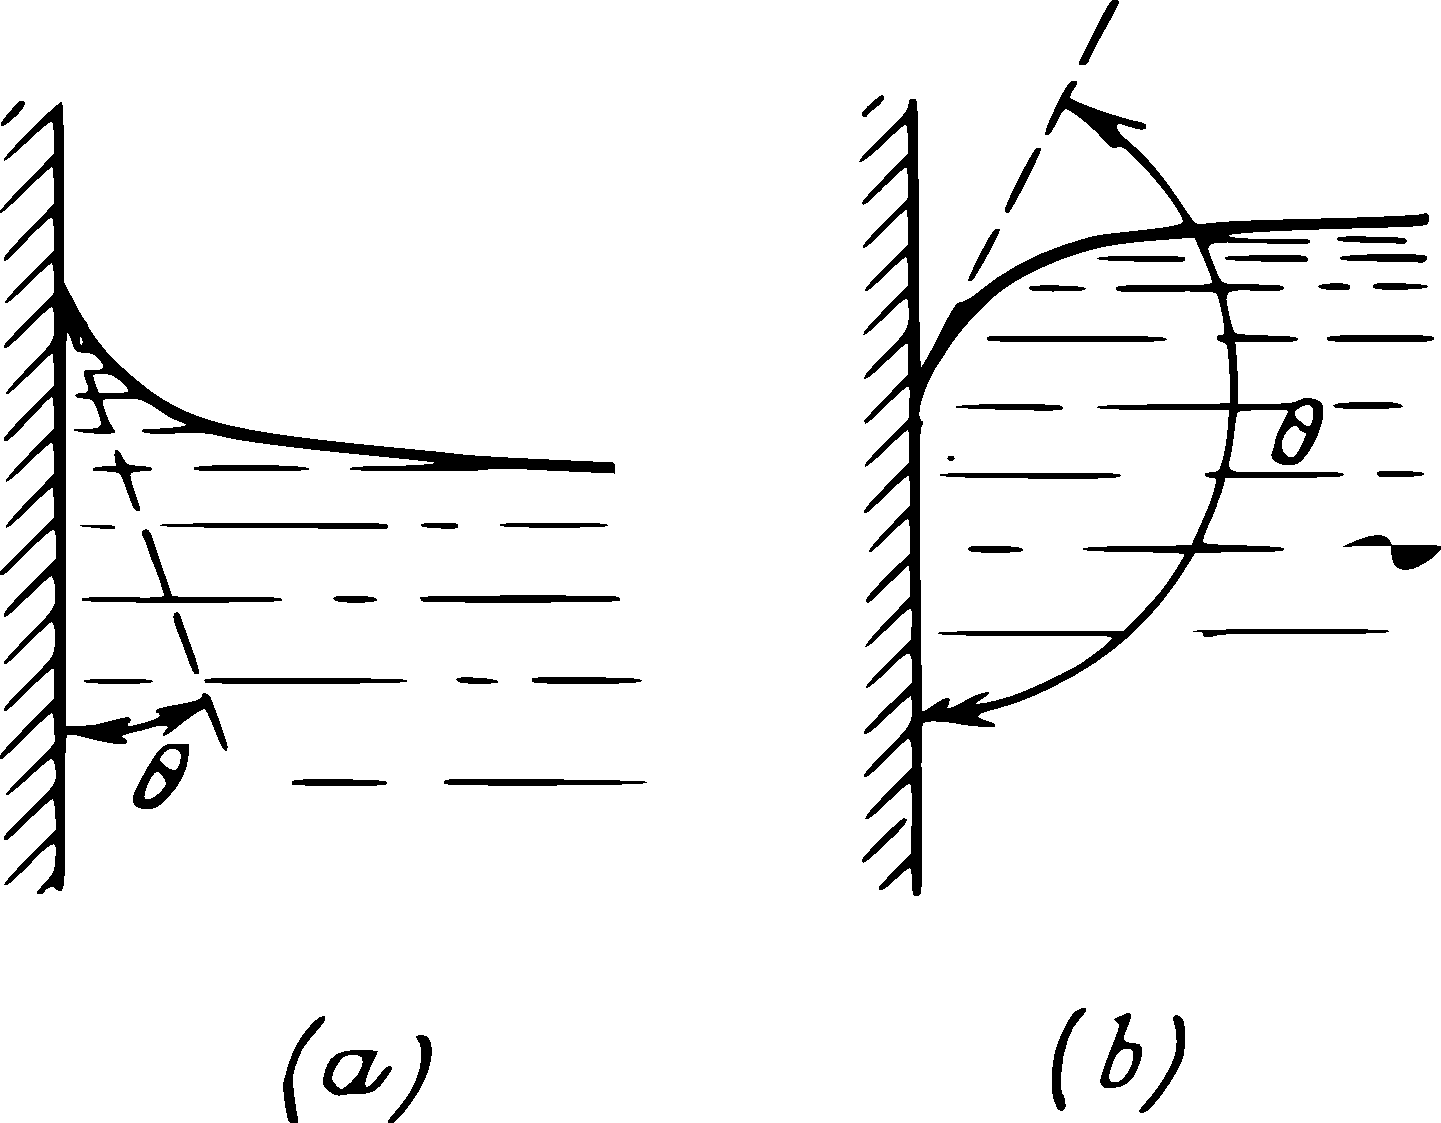
\includegraphics[width=0.75\textwidth]{figs/ch-13/fig-13-01.pdf}
\sidecaption{Angle of contact and wetting in liquids. \zhcap{液体的接触角与润湿。}\label{fig-13-01}}
\end{figure}

\section{Wetting and Capillary Phenomena}
\label{sec-13.5}
\zhtitle{润湿与毛细现象}

\subsection{}\label{13.5.1} The free surface of a liquid, curved adjacent to the wall of the vessel holding the liquid, is called the \redem{meniscus}. The line along which the meniscus contacts the wall is called the \redem{wetted perimeter}. The meniscus is characterized by the \redem{contact angle} $\theta$ between the wetted surface of the wall and the meniscus at their point of contact. When $\theta < \pi/2$ (\figr{fig-13-01}~\inred{(a)}), the liquid is said to \redem{wet} the wall(to be a \redem{wetting} liquid); when $\theta > \pi/2$ (\figr{fig-13-01}~\inred{(b)}) the liquid \redem{does not wet} the wall and is a \redem{nonwetting} liquid. 
\zhpar{液体的自由表面在靠近盛放液体的容器壁处呈弯曲状，称为\redem{弯月面}。弯月面与器壁接触的线称为\redem{湿润周界}。弯月面在接触点处由器壁表面与弯月面之间的\redem{接触角} $\theta$ 来表征。当 $\theta < \pi/2$ 时（见\figr{fig-13-01}~\inred{(a)}），称液体\redem{润湿}器壁（即为\redem{润湿性}液体）；当 $\theta > \pi/2$ 时（见\figr{fig-13-01}~\inred{(b)}），液体\redem{不润湿}器壁，即为\redem{非润湿性}液体。}



Wetting (nonwetting) is said to be ideal when $\theta = 0 \, (\theta = \pi)$. Here the meniscus is of spherical shape and is concave or convex. The absence of both wetting and nonwetting corresponds to the condition $\theta = \pi/2$, in which case the liquid has a plane free surface.
\zhpar{当 $\theta = 0$（$\theta = \pi$）时，称润湿（非润湿）为理想的。此时弯月面为球面形，呈凹形或凸形。既不润湿也不非润湿的情形，对应于 $\theta = \pi/2$ 的条件，此时液体具有平面形自由表面。}
\begin{marginfigure}[-3cm]
\centering
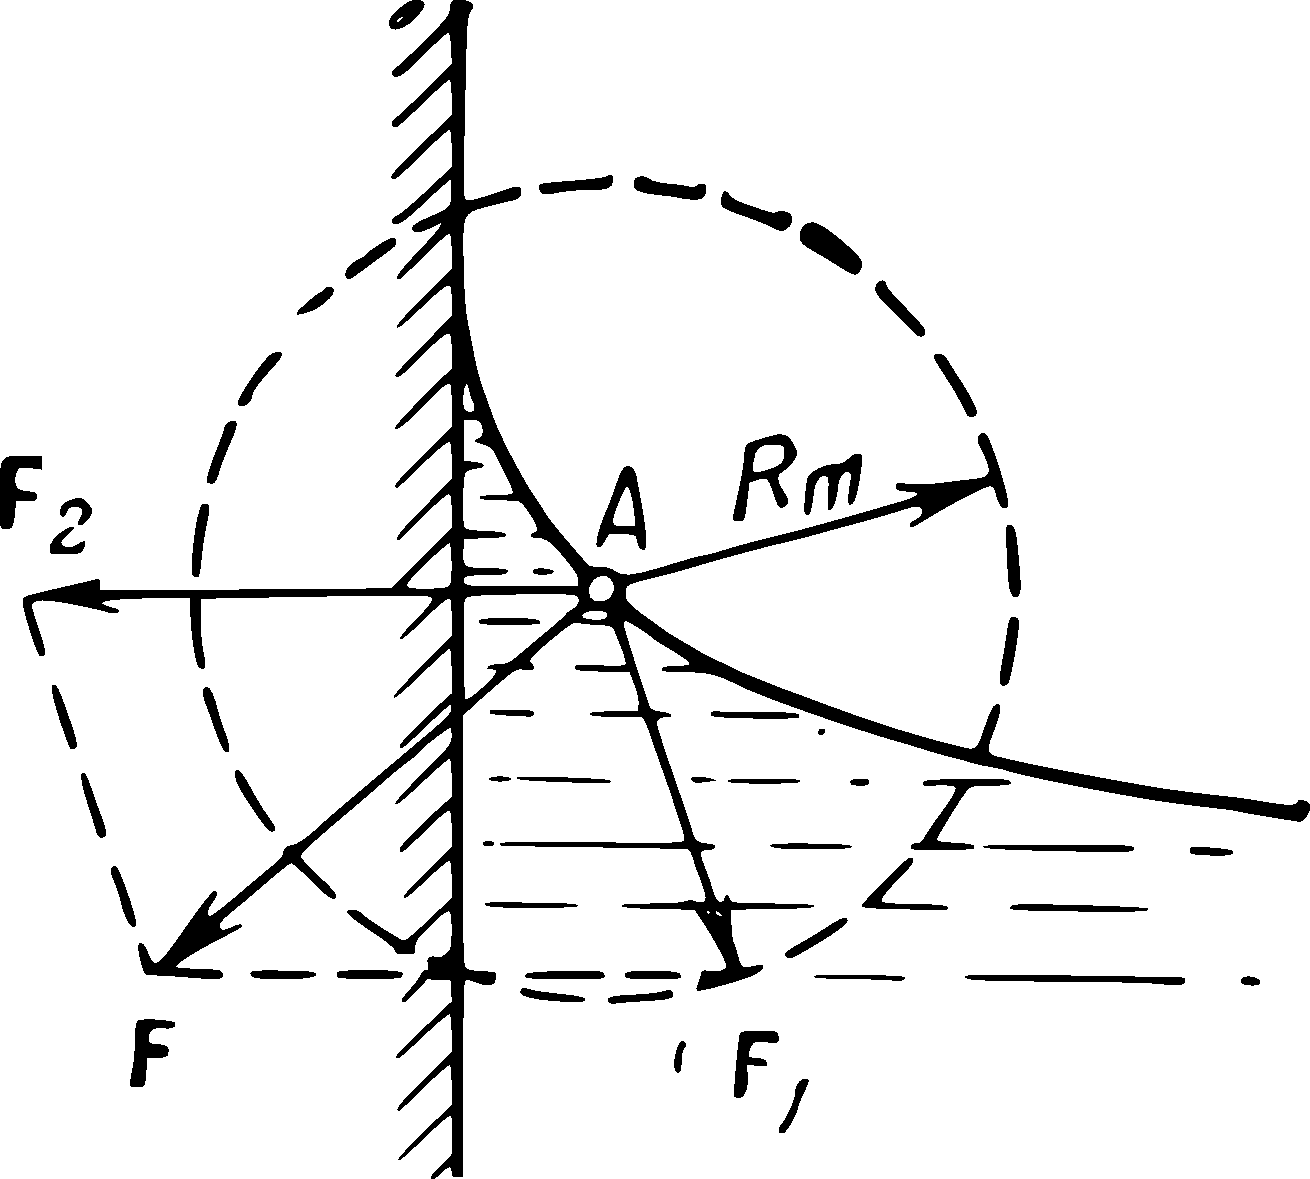
\includegraphics[width=0.8\textwidth]{figs/ch-13/fig-13-02.pdf}
\sidecaption{Range of molecular attraction. \zhcap{分子引力的作用范围。}\label{fig-13-02}}
\end{marginfigure}

\subsection{}\label{13.5.2} The formation of a meniscus is due to the interaction of the molecules with one another and with the particles of the rigid body (wall). Molecule $A$ of the surface layer, located close to the wall of the vessel and having a sphere of molecular action \ssect{12.2.3} of radius $R_{m}$ (range of molecular action) (\figr{fig-13-02}), is subject to the resultant force of attraction exerted on it by all the other molecules of the liquid $(\vb{F}_{1})$ and by all the particles of the wall $(\vb{F}_{2})$. Force $\vb{F}_{2}$ is perpendicular to the wall. This follows from considerations of symmetry. 
\zhpar{弯月面的形成是由于分子之间以及分子与刚体（器壁）粒子之间的相互作用所致。位于器壁附近、分子作用球（参见\ssect{12.2.3}）半径为 $R_{m}$（分子作用范围，见\figr{fig-13-02}）的表面层分子 $A$，受到液体中所有其他分子对它施加的合引力 $(\vb{F}_{1})$，以及器壁所有粒子对它施加的合引力 $(\vb{F}_{2})$。根据对称性可知，力 $\vb{F}_{2}$ 垂直于器壁。}


\begin{marginfigure}[-4cm]
\centering
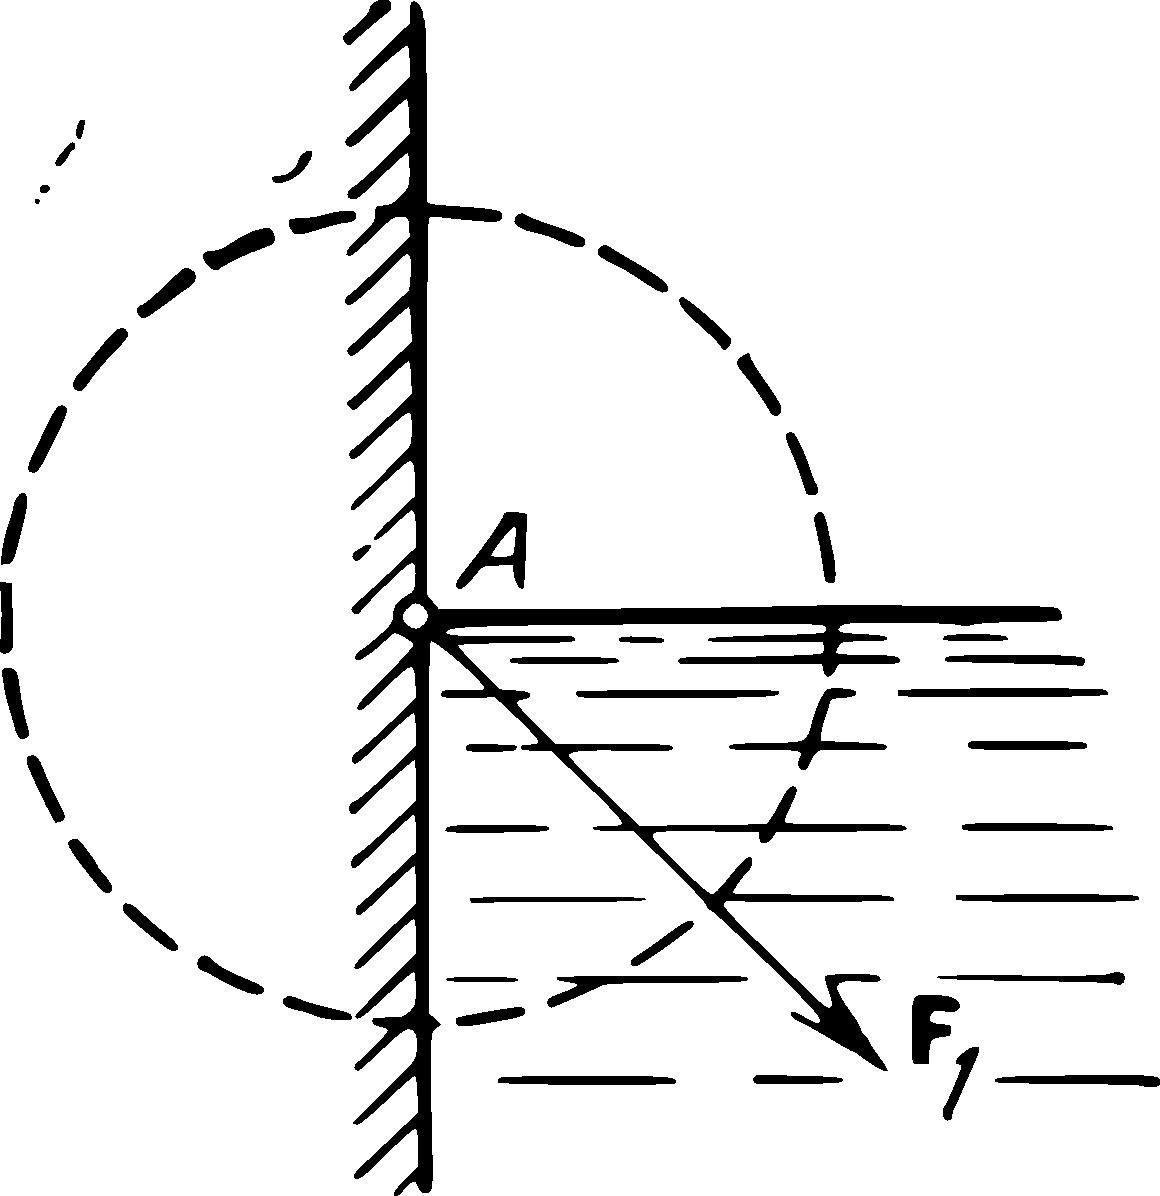
\includegraphics[width=0.8\textwidth]{figs/ch-13/fig-13-03.pdf}
\sidecaption{Range of molecular attraction. \zhcap{分子引力的作用范围。}\label{fig-13-03}}
\end{marginfigure}
The direction of force $\vb{F}_{1}$ depends upon the shape of the meniscus and the position of molecule $A$ with respect to the wall. For example, if the meniscus is flat \ssect{13.5.1} and molecule $A$ is right at the wall, force $\vb{F}_{1}$ is directed at an angle of \ang{45} to the wall (\figr{fig-13-03}). Molecule A can be in equilibrium only when the resultant force $\vb{F} = \vb{F}_{1} + \vb{F}_{2}$ is perpendicular to the surface of the liquid.\sidenote[][-1cm]{Here we ignore the gravity force acting on molecule $A$ because it is negligibly small compared to forces $\vb{F}_{1}$ and $\vb{F}_{2}$.} Otherwise, molecule $A$ would move along this surface.
\zhpar{力 $\vb{F}_{1}$ 的方向取决于弯月面的形状以及分子 $A$ 相对于器壁的位置。例如，若弯月面为平面，且分子 $A$ 恰位于器壁处，则力 $\vb{F}_{1}$ 与器壁成 \ang{45} 角（见\figr{fig-13-03}）。只有当合力 $\vb{F} = \vb{F}_{1} + \vb{F}_{2}$ 垂直于液体表面时，分子 $A$ 才能处于平衡，否则它将沿该表面移动。}
\zhpar{注：此处忽略了作用于分子 $A$ 的重力，因为它与力 $\vb{F}_{1}$ 和 $\vb{F}_{2}$ 相比小到可以忽略。}



\subsection{}\label{13.5.3} The shape of the meniscus is determined by the three possible directions of force $\vb{F}$:
\zhpar{弯月面的形状由力 $\vb{F}$ 的三种可能方向决定：}
\begin{enumerate}[label=(\alph*)]
\item force $\vb{F}$ is parallel to the surface of the wall, the liquid has a plane surface and $\theta = \pi/2$ (\figr{fig-13-04}~\inred{(a)});
\zhpar{力 $\vb{F}$ 与器壁表面平行，液体表面为平面，$\theta = \pi/2$（见\figr{fig-13-04}~\inred{(a)}）；}
\item force $\vb{F}$ is directed towards the wall; the forces of attraction exerted by the wall on molecule $A$ exceed the forces of attraction exerted on the molecule by all the other molecules of the liquid. The liquid has a concave meniscus with $\theta < \pi/2$, i.e. the liquid wets the wall (\figr{fig-13-04}~\inred{(b)});
\zhpar{力 $\vb{F}$ 指向器壁。器壁对分子 $A$ 的吸引力超过液体中其他分子对它的吸引力。此时液体具有凹形弯月面，$\theta < \pi/2$，即液体润湿器壁（见\figr{fig-13-04}~\inred{(b)}）；}
\item force $\vb{F}$ is directed towards the liquid; the forces of attraction exerted by the molecules of the liquid on molecule $A$
prevail over those exerted on it by the particles of the wall. The meniscus is convex with $\theta > \pi/2$, i.e. the liquid does not wet the wall (\figr{fig-13-04}~\inred{(c)}).
\zhpar{力 $\vb{F}$ 指向液体内部。液体中分子对分子 $A$ 的吸引力超过器壁粒子对它的吸引力。此时弯月面为凸形，$\theta > \pi/2$，即液体不润湿器壁（见\figr{fig-13-04}~\inred{(c)}）。}
\end{enumerate}


\begin{figure}[h]
\centering
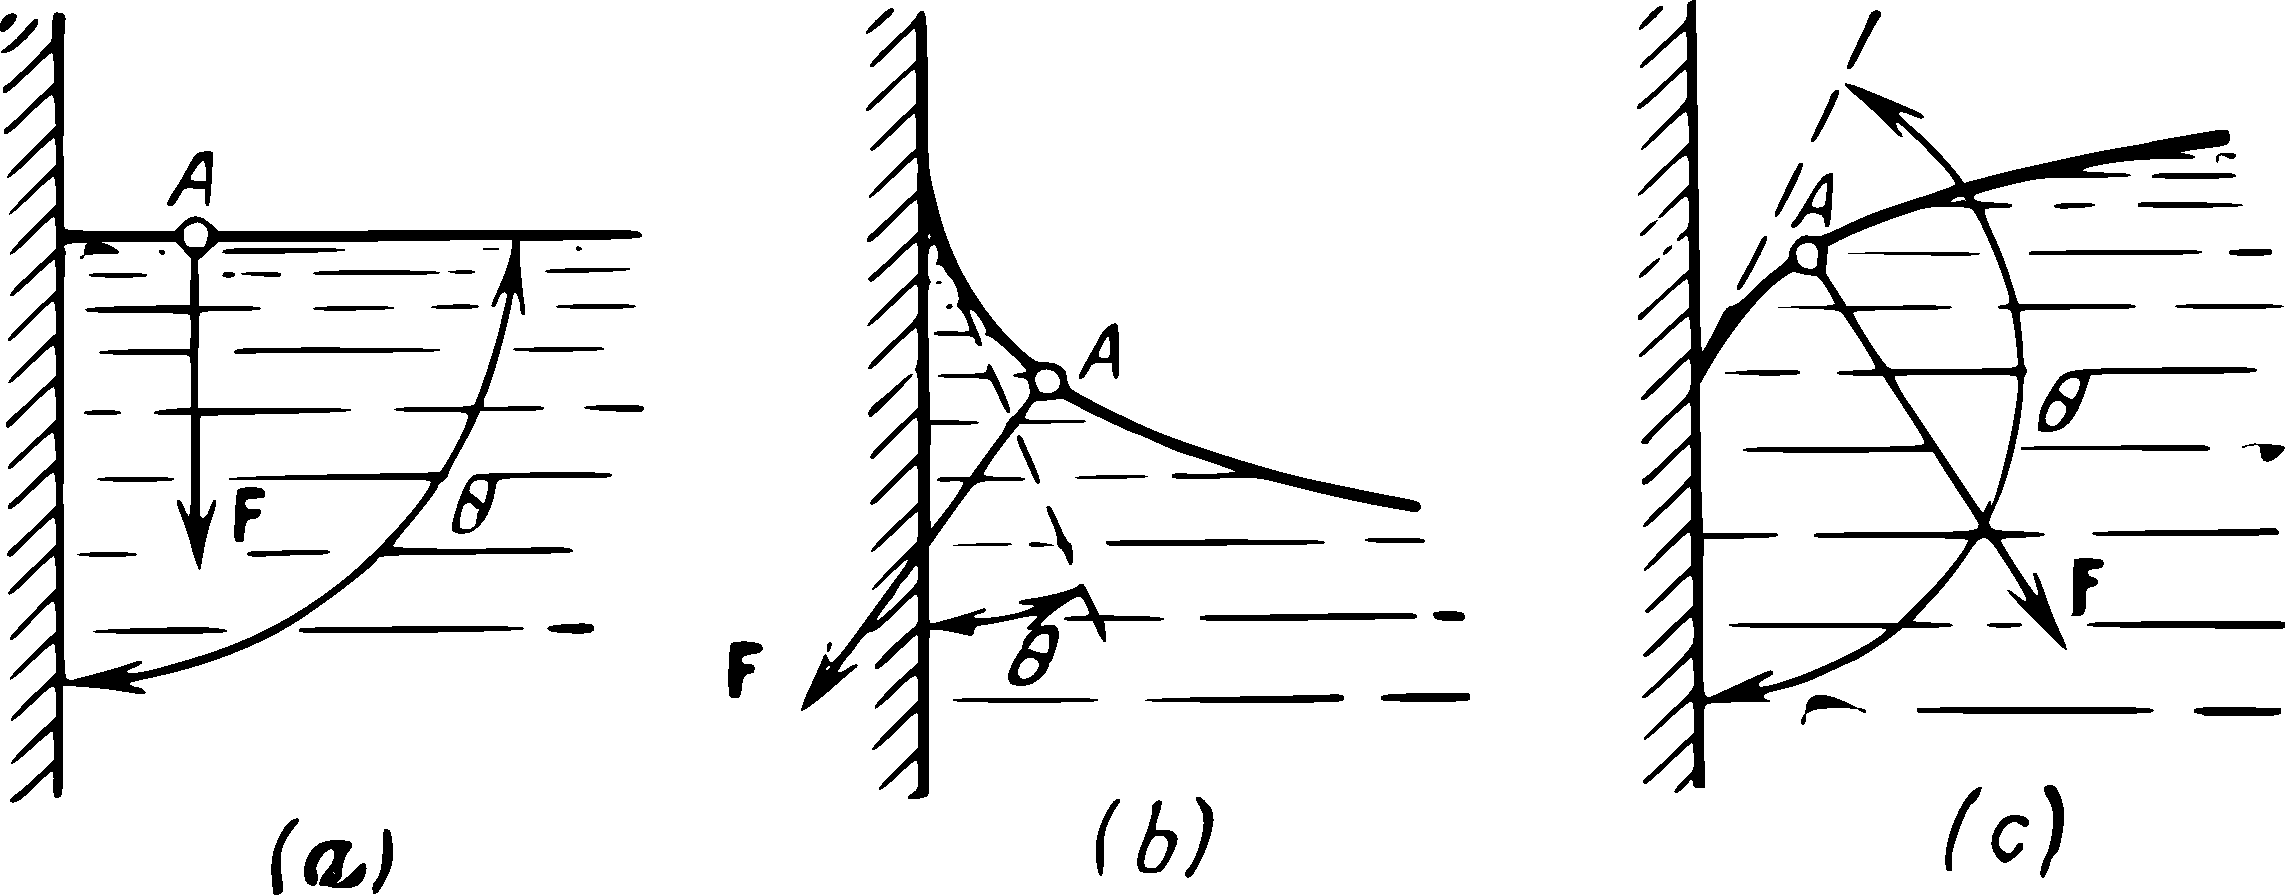
\includegraphics[width=0.9\textwidth]{figs/ch-13/fig-13-04.pdf}
\sidecaption{The shape of meniscus. \zhcap{弯月面的形状。}\label{fig-13-04}}
\end{figure}

\subsection{}\label{13.5.4} The curved shape of the surface layer is the cause of the pressure $\Delta p$, additional to the external pressure, acting on the liquid. This additional pressure is due to the surface tension. This is similar to the way in which a stretched elastic envelope (like a rubber balloon) exerts pressure on the gas it contains.
\zhpar{弯曲的表面层使液体受到一个附加于外部压强的压强 $\Delta p$，这是表面张力所致。这与受拉伸的弹性包膜（如橡皮气球）对其所包容的气体施加压强的情形类似。}

The additional pressure exerted on a liquid with a surface layer of arbitrary shape is calculated by the equation 
\zhpar{对于表面层形状任意的液体，其附加压强由下式计算：}
\begin{equation*}%
\Delta p = \sigma \left(\frac{1}{R_{1}} + \frac{1}{R_{2}}  \right)
\end{equation*}
where $\sigma$ is the surface tension \ssect{13.4.4}, and $R_{1}$ and $R_{2}$ are the radii of curvature of any two mutually perpendicular normal sections\sidenote{A normal section of the surface through point $A$ is the curve obtained as the intersection of the surface and a plane passed through the normal to the surface at this point. Radii $R_{1}$ and $R_{2}$ are called the principal radii of curvature of the surface layer.} of the surface of the liquid at the point where molecule $A$ is located. The radius of curvature $R_{1}$ (or $R_{2}$) is taken positive if its centre in the corresponding section is inside the liquid. Otherwise, the radius of curvature is taken to be negative. Thus, $\Delta p > 0$ when the meniscus is convex and $\Delta p < 0$ when it is concave. In the case of a plane surface $R_{1} = R_{2} = \infty$, and there is no additional pressure ($\Delta p = 0$). The preceding equation is called the Laplace theorem. For a spherical surface $R_{1} = R_{2 }= R$ and $\Delta p = 2\sigma/R$. Such a surplus pressure exists, for instance, within a bubble of gas of radius $R$, located inside a liquid near the surface.
\zhpar{式中 $\sigma$ 为表面张力（参见\ssect{13.4.4}），$R_{1}$ 和 $R_{2}$ 为液体表面在分子 $A$ 所在点处任意两个相互垂直的法截面的曲率半径。若某一截面中曲率半径的圆心位于液体内部，则该曲率半径取正值，否则取负值。因此，弯月面为凸形时 $\Delta p > 0$，为凹形时 $\Delta p < 0$。对于平面，$R_{1} = R_{2} = \infty$，附加压强为零（$\Delta p = 0$）。上式称为拉普拉斯定理。对于球面，$R_{1} = R_{2} = R$，$\Delta p = 2\sigma/R$。这种附加压强例如存在于靠近液体表面、位于液体内部的半径为 $R$ 的气泡之中。}
\zhpar{注：通过点 $A$ 的法截面是指表面与通过该点法线的平面相交所得的曲线。半径 $R_{1}$ 和 $R_{2}$ 称为表面层的主曲率半径。}

The surplus pressure inside a soap bubble of radius $R$ is due to the action of both superficial layers of the thin spherical film of soap (inside and outside the bubble). Thus $\Delta p = 4\sigma/R$. 
\zhpar{肥皂泡内的附加压强是由球形薄肥皂膜的两个表面层（泡内与泡外）共同作用所致。因此 $\Delta p = 4\sigma/R$。}

\subsection{}\label{13.5.5} The level of a liquid in narrow cylindrical vessels (\redem{capillary tubes}) of radius $r$ differs from the level of the liquid in a larger vessel into which the capillary tube is placed vertically. The level in the capillary tube is higher (lower) than in the larger vessel by the amount $h$ if the liquid wets (does not wet) the walls of the vessel. Here
\zhpar{在窄圆柱形容器（\redem{毛细管}）中，液面高度与将毛细管竖直插入其中的较大容器中的液面高度不同，毛细管的半径为 $r$。若液体润湿（不润湿）器壁，则毛细管中的液面高于（低于）较大容器中的液面，高度差为 $h$。其关系式为：}
\begin{equation*}%
h = \frac{2 \sigma \cos \theta}{r g \rho},
\end{equation*}
where $\theta$ is the contact angle \ssect{13.5.1}, $\rho$ is the density of the liquid, and $g$ is the acceleration due to gravity \ssect{7.3.3}. This is called \redem{Jurin's rule}.
\zhpar{式中 $\theta$ 为接触角（参见\ssect{13.5.1}），$\rho$ 为液体的密度，$g$ 为重力加速度（参见\ssect{7.3.3}）。此式称为\redem{尤林定律}。}

If the liquid is in a narrow slit of constant width $\delta$ between two parallel plates, the meniscus is of cylindrical shape having the radius $\delta/2$ and the level in the slit is above (for a wetting liquid) or below (for a nonwetting liquid) the level in the vessel in which the plates are immersed by the amount
\zhpar{若液体处于宽度为 $\delta$ 的窄缝中，窄缝由两块平行平板构成，弯月面为半径为 $\delta/2$ 的圆柱面，则缝内液面高于（润湿液体）或低于（非润湿液体）平板所浸入容器中的液面，其高度差为：}
\begin{equation*}%
h = \frac{2 \sigma \cos \theta}{\delta g \rho},
\end{equation*}

\subsection{}\label{13.5.6} The pressure of saturated vapour \ssect{12.3.2} above the curved surface of a liquid depends upon the shape of the meniscus. If the meniscus is concave (convex), the pressure of the saturated vapour is less (greater) than that above a plane surface by the amount $\Delta p_{\text{ms}}$:
\zhpar{饱和蒸气（参见\ssect{12.3.2}）在液体弯曲表面上方的压强取决于弯月面的形状。若弯月面为凹形（凸形），则饱和蒸气的压强比平面上方的压强小（大）$\Delta p_{\text{ms}}$，其值为：}
\begin{equation*}%
\Delta p_{\text{ms}} = \frac{\rho}{\rho_{1} - \rho} \, \Delta p,
\end{equation*}
where $\rho$ is the density of the saturated vapour, $\rho_{1}$ is the density of the liquid, and $\Delta p$ is the additional pressure due to the curvature of the surface \ssect{13.5.4}.
\zhpar{式中 $\rho$ 为饱和蒸气的密度，$\rho_{1}$ 为液体的密度，$\Delta p$ 为液面弯曲所引起的附加压强（参见\ssect{13.5.4}）。}

\section{Vaporization and Boiling of Liquids}
\label{sec-13.6}
\zhtitle{液体的汽化与沸腾}

\subsection{}\label{13.6.1} \redem{Vaporization}, or \redem{evaporation}, is the process of vapour formation at the free surface of a liquid. It takes place at any temperature and increases as the temperature is raised. There are molecules in the surface layer of a liquid that have high velocities and kinetic energies of thermal motion. The escape of such molecules from the surface into the space above the liquid is the explanation for evaporation with the consequent reduction of the store of internal energy and cooling of the liquid. A measure of the process of vaporization is the \redem{rate of evaporation} $u$, which is the amount of liquid converted into vapour in unit time. The rate $u$ depends upon the external pressure and the motion of the gaseous phase above the free surface of the liquid. Thus
\zhpar{\redem{汽化}，或\redem{蒸发}，是在液体自由表面形成蒸气的过程。它在任何温度下都会发生，并随温度升高而加剧。液体表面层中存在速度较大、热运动动能较大的分子。这些分子从表面逸入液面上方的空间，就是蒸发的原因，其结果是液体内能减少、液体降温。汽化过程的度量为\redem{蒸发速率} $u$，即单位时间内转化为蒸气的液体质量。速率 $u$ 取决于外部压强，以及液体自由表面上方气相的运动。由此有：}
\begin{equation*}%
u = \frac{cA}{p_{0}} \, (p_{v} - p),
\end{equation*}
where $c$ is a constant, $A$ is the area of the free surface of the liquid, $p_{v}$ is the pressure of saturated vapour, $p$ is the pressure of the vapour above the free surface of the liquid being vaporized, and $p_{0}$ is the external barometric pressure.
\zhpar{式中 $c$ 为常量，$A$ 为液体自由表面的面积，$p_{v}$ 为饱和蒸气的压强，$p$ 为正在汽化的液体自由表面上方蒸气的压强，$p_{0}$ 为外部大气压强。}


\subsection{}\label{13.6.2} \redem{Boiling} is the process of intense vaporization of a liquid, not only from its free surface, but throughout the whole volume of the liquid within the bubbles of vapour that are produced in boiling. The bubbles of vapour in a boiling liquid rapidly increase in size, rise to the surface and burst. This causes the turbulence in a boiling liquid. The pressure $p$ within a bubble of vapour located within the liquid is the sum of the external pressure $p_{0}$, the hydrostatic pressure pi of the overlying layers of liquid, and the additional pressure $\Delta p$ due to the surface tension \ssect{13.5.4}. Thus
\zhpar{\redem{沸腾}是液体的剧烈汽化过程，它不仅发生在自由表面，还发生在整个液体体积之内，即发生在沸腾过程中产生的蒸气泡之中。沸腾液体中的蒸气泡迅速增大，上升至表面并破裂，这引起了沸腾液体的湍动。位于液体内部的蒸气泡内的压强 $p$，等于外部压强 $p_{0}$、上方各液层的静水压强 $p_{1}$，以及由表面张力引起的附加压强 $\Delta p$（参见\ssect{13.5.4}）之和，即：}
\begin{align*}%
p & = p_{0} + p_{1} + \Delta p  \qand \\
p_{1} & = \rho gh, \qand \Delta p = \frac{2 \sigma}{r},
\end{align*}
where $r$ is the radius of the vapour bubble, $h$ is the distance from its centre to the surface of the liquid, and $p$ and $\sigma$ are the density and surface tension of the liquid.
\zhpar{式中 $r$ 为蒸气泡的半径，$h$ 为其中心到液体表面的距离，$p$ 和 $\sigma$ 分别为液体的密度和表面张力。}

The boiling of a liquid begins at the temperature at which the pressure $p_{v}$ of the saturated vapour inside a bubble is at least as high as the pressure $p$ \ssect{13.6.2}:
\zhpar{液体开始沸腾的温度，是使气泡内饱和蒸气压强 $p_{v}$ 至少不低于压强 $p$（参见\ssect{13.6.2}）的温度，即：}
\begin{equation*}%
p_{v} \geqslant p_{0} + \rho gh + \frac{2 \sigma}{r}.
\end{equation*}
If this condition is not complied with, the bubble collapses and the vapour it contains is condensed.
\zhpar{若该条件不满足，气泡将塌缩，其中所含的蒸气凝结。}

\subsection{}\label{13.6.3} With small radii $r$ of the vapour bubbles, the pressure $p_{v}$ should be quite high and it is necessary to heat the liquid to a high temperature before it starts boiling. If the liquid contains \redem{centres of vaporization} (dust specks, bubbles of dissolved gases, etc.), boiling begins at a much lower temperature. This is due to the fact that the vapour bubbles that appear on the centres of vaporization are of such a size that the effect of the third member in the inequality of \ssect{13.6.2} can be neglected. More­ over, $\rho gh \ll p_{0}$ as a rule, so that the approximate condition for the beginning of boiling can be written in the form
\zhpar{当蒸气泡的半径 $r$ 很小时，蒸气压强 $p_{v}$ 应当很高，因此必须将液体加热到很高的温度才会开始沸腾。若液体中含有\redem{汽化核心}（尘埃微粒、溶解气体的气泡等），沸腾则会在低得多的温度下开始。这是因为，在汽化核心上出现的蒸气泡尺寸合适，使得\ssect{13.6.2}中不等式的第三项的影响可以忽略不计。此外，通常 $\rho gh \ll p_{0}$，因此沸腾开始的近似条件可以写成如下形式：}
\begin{equation*}%
p_{v} \approx  p_{0}.
\end{equation*}
The temperature of a liquid at which the pressure of its saturated vapour is equal to the external pressure is called the \redem{boiling point} of the liquid.
\zhpar{使饱和蒸气压强等于外部压强的液体温度，称为该液体的\redem{沸点}。}

\subsection{}\label{13.6.4} When a liquid boils at constant pressure, its temperature remains constant. The quantity of heat transferred to a boiling liquid is completely expended in converting the molecules of the liquid into vapour. The heat $r_{b}$ required to vapor­ize unit mass of a liquid heated to the boiling point is called the \redem{heat of vaporization}. The value of $r_{b}$ decreases as the boiling point is raised and vanishes at the critical temperature \ssect{12.3.1}.
\zhpar{液体在恒定压强下沸腾时，其温度保持不变。传给沸腾液体的热量全部用于使液体分子转化为蒸气。将已加热到沸点的单位质量液体转化为蒸气所需的热量 $r_{b}$，称为\redem{汽化热}。$r_{b}$ 的数值随沸点升高而减小，并在临界温度（参见\ssect{12.3.1}）时变为零。}

The change in the internal energy of a liquid \ssect{9.1.1} as a unit of its mass is converted into vapour at the boiling point is called the \redem{internal heat of vaporization}.
\zhpar{单位质量液体在沸点下转化为蒸气时，其内能的改变量（参见\ssect{9.1.1}）称为\redem{内汽化热}。}

\subsection{}\label{13.6.5} The boiling of liquids and the condensation of vapour are examples of first-order phase transitions (cf. \ssect{12.4.2}). Typ­ical of such phase transitions are the simultaneous constant values of pressure and temperature, but the changing ratio of the masses of the two phases \ssect{12.3.3}. For a first-order phase transition to occur, the heat $r_{b}$ (\redem{specific latent heat of vaporization}) must be supplied to or taken away from the system. The heat $r_{b}$ per unit mass is calculated by the \redem{Clausius-Clapeyron equation}:
\zhpar{液体的沸腾和蒸气的凝结是一级相变的例子（参见\ssect{12.4.2}）。这类相变的典型特征是压强与温度同时保持恒定，但两相的质量比不断变化（参见\ssect{12.3.3}）。要使一级相变发生，必须向体系输入或从体系取出热量。单位质量的热量 $r_{b}$（\redem{比汽化潜热}）由\redem{克拉珀龙-克劳修斯方程}计算：}
\begin{equation*}%
r_{b} = (v_{2} - v_{1}) \, T \, \dv{p}{T},
\end{equation*}
where $v_{1}$ and $v_{2}$ are the specific volumes of the substance in the initial and final phases, $T$ and $p$ are the temperature and pressure of the phase transition.
\zhpar{式中 $v_{1}$ 和 $v_{2}$ 分别为物质在初相和末相中的比体积，$T$ 和 $p$ 分别为相变时的温度和压强。}

\subsection{}\label{13.6.6} It follows from the Clausius-Clapeyron equation for the boiling of liquids that
\zhpar{由液体沸腾的克拉珀龙-克劳修斯方程可得：}
\begin{equation*}%
\dv{T}{p} = \frac{v_{\text{v}} - v_{1}}{r_{b}},
\end{equation*}
where $v_{1}$ and $v_{\text{v}}$ are the specific volumes of the liquid and vapour at the boiling point $T$. Since $v_{\text{v}} > v_{1}$ and $r_{b} > 0$, $\dv*{T}{p} > 0$, i.e. the boiling point increases with pressure. For instance, at the pressure $p = \SI{1.25d7}{\pascal}$ water can be heated without boiling to a temperature at which lead can be melted in the water. The melting point of lead is \SI{900}{\kelvin}.
\zhpar{式中 $v_{1}$ 和 $v_{\text{v}}$ 分别为沸点 $T$ 时液体和蒸气的比体积。由于 $v_{\text{v}} > v_{1}$ 且 $r_{b} > 0$，故 $\dv*{T}{p} > 0$，即沸点随压强升高而升高。例如，在压强 $p = \SI{1.25d7}{\pascal}$ 下，水可以不沸腾地加热到能使铅在水中熔化的温度。铅的熔点为 \SI{900}{\kelvin}。}



